%%% Section start %%%
\section{Background}
\label{sec-background}
%Background  (1 p.): a) GRADE b) UFO +BDT?


\subsection{The Grade Taxonomy}
\label{subsec-taxonomy}

The GRADE taxonomy~\cite{papatheocharous2015decision,papatheocharous2018thegrade} was proposed as a tool to support the organization and characterization of the decision making process for software systems. This taxonomy is structured in five top-level elements, which are then refined in larger sets of lower-level concepts, intending to represent different decision-making aspects. Both top-level and lower-level concepts provide a common terminology to be used by researchers and practitioners to document a decision and to identify additional elements that can impact decisions in an organization. The five top-level elements proposed in the GRADE taxonomy are: 
\begin{itemize}
	\item Goals (G): represent the objectives that a decision intends to achieve;
	\item Roles (R): represent the stakeholders that are involved in the decision-making process. In the context of the taxonomy, not only people that make the decision are considered roles, but also people that will be affected by that particular decision;
	\item Assets (A): document the options that are available during the decision-making process. They are the elements that the decision maker takes into consideration to satisfy the decision goal(s);
	\item Environment (E): represents the contextual elements around the decision-making process that can be relevant, influencing and affecting the outcome of a decision. In other words, the Environment represents the situation of the world, before the decision is made;
	\item  Decision Methods and Criteria (D): catalog the ways (i.e. methods) to perform the decision-making process, and the criteria evaluated to guide such process.
\end{itemize}   

%Figure~\ref{fig-grade-taxonomy} presents an overview of elements that compose the GRADE taxonomy.
%
%\begin{figure}
%	\centering
%	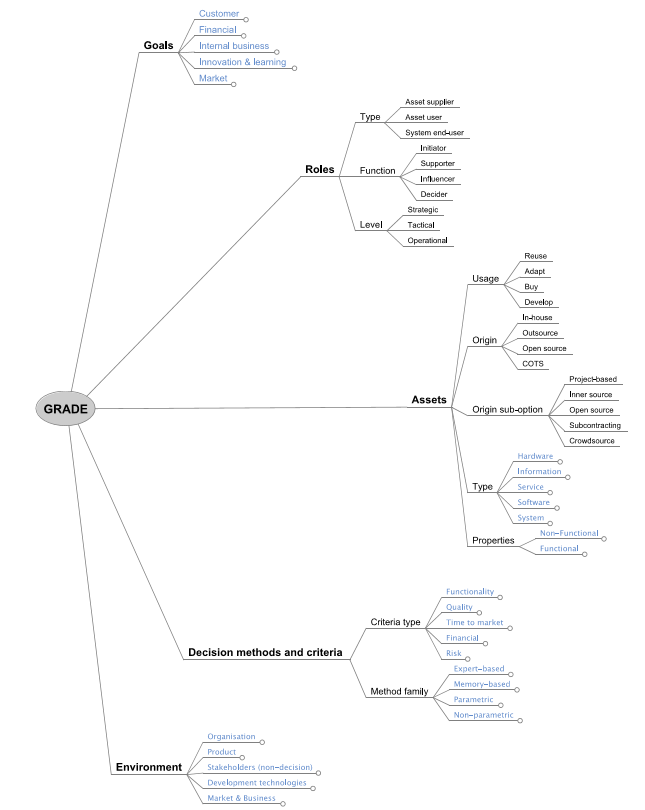
\includegraphics[width=\textwidth]{figuras/fig-grade-taxonomy} 
%	\caption{An overview of the Grade Taxonomy~\cite{papatheocharous2018thegrade}.}
%	\label{fig-grade-taxonomy}
%\end{figure}

The GRADE taxonomy is built for a specific decision-making sub-domain, its elements are specializations of Basic Decision Theory (BDT)~\cite{decision-theory} concepts, i.e. acts, events, outcomes, and payoffs. Therefore, in order to provide a precise semantic account of the concepts composing the GRADE taxonomy, it is essential to understand well the BDT elements.

In BDT, acts are the actions considered by the agent. For instance, when leaving, the agent can ``carry the umbrella'' or ``not carry the umbrella''. Events are occurrences beyond the control of the agent, e.g., the possibility of rain. Outcomes are the result of the occurrence of acts and events. For example, ``getting wet or not'' and ``carrying or not the weight of the umbrella''. Payoffs are judgments of value that the decision maker makes for each outcome. For example, how much is it worth being free from the bother of carrying an umbrella in face of the possibility of rain?


\subsection{Decision-making Ontology}
\label{subsec-decision-making}

The Decision-making Ontology (DMO)~\cite{guizzardi2018aligning} is a core ontology composed of the basic concepts underlying the decision-making process. DMO is grounded on the UFO foundational ontology~\cite{guizzardi:phdthesis05}, thus reusing and specializing UFO concepts. Figure~\ref{fig-decision-making-ontology} presents DMO's conceptual model.

\begin{figure}
	\centering
	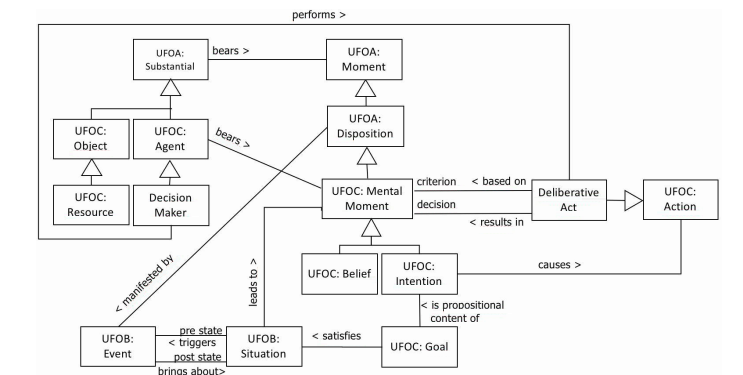
\includegraphics[width=\textwidth]{figuras/fig-decision-making-ontology} 
	\caption{The Decision-Making Ontology~\cite{guizzardi2018aligning} conceptual model.}
	\label{fig-decision-making-ontology}
\end{figure}

In DMO, a \textit{Deliberative Act} is an \textit{Action} performed by a \textit{Decision-Maker}, which is the \textit{Agent} responsible for making a \textit{Decision}. In its turn, a \textit{Decision} is a \textit{Mental Moment} (more specifically, an \textit{Intention} or a \textit{Belief}) that inheres in (being existentially dependent on) the \textit{Decision-Maker}. Additionally, the Decision-Maker may use some criteria to make a decision. A \textit{Criterion} is also a \textit{Mental Moment} of the \textit{Decision Maker}. Finally, it is important to explain that the \textit{Goal} aimed by \textit{Decision-Maker} when executing the \textit{Deliberative Act} attempts to achieve a particular \textit{Situation} of the world. In other words, the \textit{Decision-Maker} attempts to change the state of the world from a Situation A to a Situation B, which is compliant with his \textit{Intention}.

